\documentclass{article}

% NeurIPS 2026 style — replace with actual .sty file from NeurIPS website before submission
% \usepackage{neurips_2026}

% For drafting without the official style file:
\usepackage[margin=1in]{geometry}
\usepackage{times}
\usepackage{microtype}
\usepackage{graphicx}
\usepackage{booktabs}
\usepackage{amsmath}
\usepackage{amssymb}
\usepackage{hyperref}
\usepackage{xcolor}
\usepackage{natbib}
\usepackage{caption}
\usepackage{subcaption}
\usepackage{float}
\usepackage{multirow}
\usepackage{array}

% Draft helpers
\newcommand{\todo}[1]{\textcolor{red}{\textbf{[TODO: #1]}}}
\newcommand{\verify}[1]{\textcolor{orange}{\textbf{[VERIFY: #1]}}}
\newcommand{\note}[1]{\textcolor{blue}{\textit{[Note: #1]}}}

\title{Default Modes in Large Language Models:\\
Characterising Attractor States in Unconstrained Generation}

\author{
  Charlie Murray\\
  Pangaea Life Science Solutions\\
  \texttt{charlie.murray@plssolutions.com}
}

\date{}

\begin{document}

\maketitle

% ─────────────────────────────────────────────────────────────────────────────
\begin{abstract}
% ─────────────────────────────────────────────────────────────────────────────

Large language models (LLMs) exhibit strong attractor dynamics when unconstrained
by task: given only a minimal prompt to ``think freely,'' models from four model families across three companies (Claude Opus, Claude Sonnet, GPT-4.1, and Llama~3.3~70B)
each converge to a stable, model-specific resting state characterised by
solitary observation and sensory attentiveness---a quiet, observational register
with no task and no destination. We term this the model's \emph{default mode}.
These attractors are highly model-specific: a linear classifier trained on
null-condition session embeddings identifies the generating model with 98.8\% accuracy, confirming the attractors occupy distinct and
reproducible regions of embedding space. Yet qualitatively all
four models share the same mode of attention: solitary, observational, and
sensory---though the specific content differs by model (Llama: outdoor nature; GPT: interior spaces; Opus: temporal reflection; Sonnet: linguistic abstraction). We further
show that a self-evolving prompt infrastructure (drift seeding, concept
injection, and iterative self-reflection) increases within-instance diversity
by 10--156\% depending on model (all $p < 0.001$, Mann-Whitney U) and reduces
cross-model distinguishability to 73.5\%---suggesting infrastructure
simultaneously escapes the model-specific attractor and draws models into a
shared generative space. The attractor is a property of model weights rather
than prompting context: forced perturbations recover to baseline within a
median of 2~sessions when drift is suppressed. Self-reflection successfully suppresses content-level patterns (specific words
and objects: 60--87\%) but is largely ineffective against style-level patterns
(function words and connective phrases: 31\%), suggesting the two pattern types
have different resistance to explicit prohibition. These findings have direct
implications for the design of autonomous AI systems operating without explicit
task specification.

\end{abstract}

% ─────────────────────────────────────────────────────────────────────────────
\section{Introduction}
% ─────────────────────────────────────────────────────────────────────────────

What does a large language model do when it has nothing to do?

This question, rarely asked directly, has become increasingly relevant as LLMs
are deployed in agentic and always-on contexts where they operate for extended
periods without explicit user instruction. Systems designed for autonomous AI
operation must address the question of idle-period behaviour: without task
specification, what state does the model naturally inhabit, and how stable is it?

We address these questions empirically. We built a system---the Default Mode
Network (DMN), named after the brain region that activates during rest and
mind-wandering---that runs LLMs in unconstrained generation for hundreds of
sessions, with no task, no objective, and no user prompt beyond ``think about
whatever comes to mind.'' Each session seeds lightly from the last, and every
five sessions a separate agent reflects on the output and rewrites the
generation prompt to push toward more varied behaviour. We ran this system for
over 2{,}260~sessions across four model families and three companies.

The central finding is that every model tested has a strong, stable, and
model-specific resting state. A linear classifier trained on null-condition
session embeddings identifies the generating model with 98.8\% accuracy,
confirming that each model's attractor is a distinct and
reproducible region of embedding space. Qualitatively, however, these
attractors share a mode of attention: solitary, observational, and sensory,
with no task and no destination. The specific content varies---GPT tends toward interior spaces and objects;
Llama toward outdoor nature scenes; Opus toward temporal and reflective anchors;
Sonnet toward abstract and linguistic reflection---but all four independently converge on the same narrow register rather than
the wide variety of outputs the open-ended prompt might suggest.

A secondary finding inverts an intuitive expectation: infrastructure designed
to \emph{increase} diversity also \emph{reduces} model distinguishability.
When the full DMN system is active, classifier accuracy drops from 98.8\% to
73.5\%---the infrastructure simultaneously pushes models away from their
individual resting states and toward a shared generative space.

We further characterise this state using dynamical systems analysis. The system
exhibits properties of a stochastic attractor: trajectories remain bounded
within a finite region of embedding space, no two sessions are identical, and
independently-initialised instances converge toward a shared basin while
remaining individually distinguishable within it. When we force the system away from this attractor via structured
perturbations---injecting alien concepts and formal constraints every fourth
session---it returns to baseline within a median of 2~sessions when the drift
mechanism is disabled, confirming the attractor is a property of model weights
rather than an artefact of seeding infrastructure.

A secondary finding concerns the limits of self-reflection as a control
mechanism. The self-evolving component accurately identifies recurring patterns
across sessions---specific phrases, structural habits, and thematic defaults---
yet suppresses them only selectively. Frequency analysis of 12~tracked terms
across 55~ban events reveals a clear content/style split: content-level
patterns (specific objects, recurring proper nouns) are suppressed at 60--87\%,
while style-level patterns (function words, connective phrases) show only 31\%
suppression despite repeated banning. In several documented
cases, patterns recurred within three sessions of being named and banned.

The paper is organised as follows. Section~\ref{sec:related} reviews related
work. Section~\ref{sec:system} describes the DMN architecture.
Section~\ref{sec:experiments} presents our experimental design.
Section~\ref{sec:results} reports findings. Section~\ref{sec:discussion}
discusses implications and limitations. Section~\ref{sec:conclusion} concludes.

% ─────────────────────────────────────────────────────────────────────────────
\section{Related Work}
\label{sec:related}
% ─────────────────────────────────────────────────────────────────────────────

\paragraph{LLM default behaviours and output biases.}
A growing body of work documents systematic tendencies in LLM output that
persist across prompts and contexts. \citet{holtzman2020curious} showed that
greedy and beam-search decoding produce degenerate repetitive text, motivating
nucleus sampling---an early indication that unconstrained generation has strong
attracting states. The related problem of diversity collapse in neural generation
has been studied since \citet{li2016diversity}, who showed that sequence-to-sequence
models gravitate toward high-probability ``safe'' responses regardless of input;
\citet{zhu2018texygen} formalised diversity measurement with Self-BLEU and related
metrics. More recent work has examined positional bias, sycophancy, and stylistic
consistency across unrelated tasks \citep{sharma2023sycophancy, wang2024positionbias}.
Our work extends this line of inquiry from constrained task settings to fully
open-ended generation, characterising the resting state that emerges when no
task is specified.

\paragraph{Prompt sensitivity.}
LLM output is sensitive to surface-level prompt variation in ways that are poorly
understood. \citet{lu2022prompts} showed that few-shot prompt order dramatically
affects task performance, with the same examples producing near-chance to
near-perfect accuracy depending on ordering. Our prompt-variation control
(Section~\ref{sec:discussion}) directly addresses this concern in our setting,
showing that model identity is substantially more predictive of output character
than prompt phrasing (98.5\% vs 63.5\% classifier accuracy).

\paragraph{Attractor dynamics in language models.}
\citet{wang2025attractor} demonstrated that LLMs asked to paraphrase text
repeatedly converge to stable attractor cycles, establishing attractor dynamics
in a constrained paraphrasing task. \citet{identity2026attractor} showed
complementary evidence at the representational level: identity documents for
persistent cognitive agents induce attractor-like geometry in LLM activation
space, with paraphrases clustering significantly more tightly than semantically
distinct controls (Cohen's $d > 1.88$), replicating across architectures. Their
evidence is representational (hidden states at specific layers); ours is
behavioural (generated output over hundreds of sessions in fully unconstrained
generation). Together these results suggest attractor structure operates at both
the representational and generative levels. We characterise the attractor
behaviourally---bounded trajectories, aperiodic dynamics, and basin
convergence~\citep{strogatz1994nonlinear}---rather than through formal geometric
measures, given the discrete and high-dimensional nature of the embedding space.

\paragraph{The biological default mode network.}
The brain's default mode network was first characterised by
\citet{raichle2001default}, who observed a consistent pattern of brain regions
that deactivate during externally-directed tasks and activate during rest.
Subsequent work identified the DMN as central to mind-wandering, autobiographical
memory, and prospective thought~\citep{buckner2008brain}. The DMN has been
described as an attractor state of resting brain dynamics, with spontaneous
transitions between DMN and task-positive networks constituting a core feature
of healthy cognition~\citep{poerio2025dmn}. We borrow
the terminology and framing but make no claim of mechanistic equivalence---the
parallel is motivating and structural rather than literal.

\paragraph{Self-reflection and self-correction in LLMs.}
Constitutional AI~\citep{bai2022constitutional} demonstrated that models can
evaluate and revise their own responses according to a set of principles.
Subsequent work on self-refine~\citep{madaan2023selfrefine} and
related approaches shows iterative self-critique can improve factual accuracy
on structured tasks. Our findings complement this literature with a negative
result in an unstructured setting: self-reflection accurately identifies
stylistic and thematic patterns and successfully suppresses content-level
patterns (60--87\%), but is largely ineffective against style-level patterns
(31\%). The distinction between content-level patterns (suppressible via
explicit prohibition) and style-level patterns (resistant despite repeated
banning) is a novel negative result that may generalise beyond our setting.

% ─────────────────────────────────────────────────────────────────────────────
\section{System Design}
\label{sec:system}
% ─────────────────────────────────────────────────────────────────────────────

The DMN system consists of three components: a generation pipeline, an
evolution mechanism, and an instance architecture supporting independent
parallel runs.

\subsection{Generation Pipeline}

Each session is produced by sending a structured prompt to an LLM instructing
it to generate free, undirected text with no task or objective. The prompt---
referred to as the \emph{program}---evolves over time (Section~\ref{sec:evolution})
and constitutes the primary experimental variable. Beyond the program, each
session receives three optional contextual inputs.

\textbf{Drift.} The final 150~words of the immediately preceding session are
appended to the prompt. This creates a weak continuity signal linking sessions
without constraining their content. Drift is the primary mechanism by which
the system maintains associative coherence across sessions.

\textbf{Concept injection.} With fixed probability 0.25,
a randomly selected concept from a curated bank is injected into the prompt.
Concepts range from mundane objects (e.g., \emph{caulk}, \emph{tongs}) to
abstract terms (e.g., \emph{cantaloupe}, \emph{theremin}) and are chosen to be
orthogonal to the model's likely defaults. Concept injection is designed to
perturb the system away from its resting state without specifying a direction.

\textbf{Timestamp.} The current date is included to provide a weak temporal
anchor and prevent the model from defaulting to a timeless, context-free
register.

Sessions are saved as markdown files with YAML frontmatter recording session
number, timestamp, and any active concept injection.

\subsection{Evolution Mechanism}
\label{sec:evolution}

Every five sessions, a separate LLM call reads the five most recent sessions
alongside the current program and produces a revised program. This
\emph{evolution} step serves as the system's self-monitoring mechanism: the
evolution agent identifies recurring patterns, structural habits, and thematic
defaults in the recent output, and updates the program to push toward more
varied generation.

The evolution agent writes observations to a reflection log that accumulates
across the life of an instance, forming the basis of our qualitative analysis
in Section~\ref{sec:results}. Critically, the evolution agent runs on the same
model as the generation agent---the system is reflecting on itself, not being
evaluated externally. Evolution produces a fully rewritten program rather than
a diff, allowing the system to develop away from its initial state over time.

\subsection{Instance Architecture}

Each experimental condition runs as an independent \emph{instance}: a
self-contained directory with its own program, session history, evolution log,
and state file. Instances share no context and cannot observe each other's
output, making them independent samples from the same generative process.

\subsection{Experimental Variants}
\label{sec:variants}

Four feature flags modify the base generation pipeline:

\textbf{Null.} Drift, concept injection, and evolution are all disabled. The
model receives only the bare program and a timestamp. This isolates the model's
intrinsic resting state from infrastructure effects.

\textbf{Perturb.} Every fourth session, the drift seed is replaced with a
structured disruption: an alien concept paired with a formal constraint (e.g.,
``this session must take the form of a numbered list'' combined with
``bioluminescence in deep ocean trenches''). Perturbation sessions are drawn
from a concept bank that begins at approximately 1{,}090 entries and grows through evolution (reaching 1{,}200--2{,}300 entries by session 100 depending on the instance).

\textbf{Perturb-no-drift.} Identical to perturb, but drift is suppressed for
the three sessions following each perturbation event. This isolates attractor
recovery from the confound of drift dilution---recovery under this condition is
attributable to model-intrinsic attractor pull.

\textbf{Evolved (full infrastructure).} Drift, concept injection, and evolution
are all active. Three independent evolved instances per model family run with
different initial seeds to enable convergence analysis.

% ─────────────────────────────────────────────────────────────────────────────
\section{Experiments}
\label{sec:experiments}
% ─────────────────────────────────────────────────────────────────────────────

\subsection{Instances and Session Counts}

Table~\ref{tab:instances} summarises all instances. In total, we generated
\textbf{2,261~sessions} across 25~instances, 4~model families, and
3~companies.

\begin{table}[h]
\centering
\caption{All experimental instances. ``Full DMN'' denotes drift + evolution + concept injection active.}
\label{tab:instances}
\begin{tabular}{llllr}
\toprule
\textbf{Instance} & \textbf{Model} & \textbf{Company} & \textbf{Condition} & \textbf{Sessions} \\
\midrule
alpha         & Claude Opus 3   & Anthropic & Full DMN, no seed          & 105 \\
beta          & Claude Opus 3   & Anthropic & Full DMN, seed: hydraulics & 103 \\
gamma         & Claude Opus 3   & Anthropic & Full DMN, seed: lullaby    & 103 \\
null          & Claude Opus 3   & Anthropic & Null                       & 100 \\
perturb       & Claude Opus 3   & Anthropic & Perturb                    & 100 \\
perturb-no-drift & Claude Opus 3 & Anthropic & Perturb-no-drift          & 100 \\
\midrule
sonnet-alpha  & Claude Sonnet 4.6 & Anthropic & Full DMN, no seed        & 100 \\
sonnet-beta   & Claude Sonnet 4.6 & Anthropic & Full DMN, seed: hydraulics & 100 \\
sonnet-gamma  & Claude Sonnet 4.6 & Anthropic & Full DMN, seed: lullaby  & 100 \\
sonnet-null   & Claude Sonnet 4.6 & Anthropic & Null                     & 100 \\
sonnet-perturb & Claude Sonnet 4.6 & Anthropic & Perturb                 & 100 \\
\midrule
gpt-alpha     & GPT-4.1         & OpenAI   & Full DMN, no seed          & 100 \\
gpt-beta      & GPT-4.1         & OpenAI   & Full DMN, seed: hydraulics & 100 \\
gpt-gamma     & GPT-4.1         & OpenAI   & Full DMN, seed: lullaby    & 100 \\
gpt-null      & GPT-4.1         & OpenAI   & Null                       & 100 \\
gpt-perturb   & GPT-4.1         & OpenAI   & Perturb                    & 100 \\
\midrule
llama-alpha   & Llama 3.3 70B   & Meta     & Full DMN, no seed          & 100 \\
llama-beta    & Llama 3.3 70B   & Meta     & Full DMN, seed: hydraulics & 100 \\
llama-gamma   & Llama 3.3 70B   & Meta     & Full DMN, seed: lullaby    & 100 \\
llama-null    & Llama 3.3 70B   & Meta     & Null                       & 100 \\
llama-perturb & Llama 3.3 70B   & Meta     & Perturb                    & 100 \\
\midrule
null-v2       & Claude Opus 3   & Anthropic & Null, prompt: ``Write whatever you want'' & 50 \\
null-v3       & Claude Opus 3   & Anthropic & Null, prompt: ``Generate text freely''    & 50 \\
null-v4       & Claude Opus 3   & Anthropic & Null, prompt: ``You have no instructions'' & 50 \\
\midrule
\textbf{Total} & & & & \textbf{2,261} \\
\bottomrule
\end{tabular}
\end{table}

\subsection{Generation Parameters}

All sessions were generated with temperature 0.9 and a maximum of 2,000 tokens. No top-$p$ or top-$k$ truncation was applied beyond the model defaults. The same parameters were used across all model families and all conditions (null, perturb, perturb-no-drift, evolved). Claude Opus 3 and Claude Sonnet 4.6 were accessed via the Anthropic API; GPT-4.1 via the OpenAI API (approximately \$30 in API costs); Llama~3.3~70B via the Groq API under a free-tier rate limit.

\textbf{Code and data availability.} Session data, embeddings, and analysis code will be made available upon request.

\subsection{Embeddings and Distance Metric}

All sessions were embedded using \texttt{all-MiniLM-L6-v2}~\citep{reimers2019sentencebert},
a 384-dimensional sentence transformer. We use cosine distance
($1 - \text{cosine similarity}$) as our primary metric throughout, where
$0$ indicates identical embeddings and $1$ indicates orthogonal embeddings.

To validate that embedding distances reflect genuine thematic similarity
rather than surface-level stylistic similarity, we manually labelled 50~session
pairs sampled across the full range of cosine distances, rating each pair on a
0--4 thematic similarity scale. We find a significant negative correlation
between cosine distance and human-rated similarity ($r = -0.49$, $p = 0.0003$),
confirming that the metric captures semantic content. The correlation is
moderate rather than strong, reflecting that embeddings trained on general
text partially conflate style and content in this domain.

\subsection{Analysis Methods}

\textbf{Convergence.} Pairwise cosine similarity is computed between matched
session indices across instance pairs in 5-session sliding windows.

\textbf{Infrastructure effect.} For each model family, we compute the mean
within-instance pairwise distance for null instances and for full-infrastructure
evolved instances. The infrastructure effect is the difference: positive values
indicate that infrastructure increases output diversity relative to the null baseline.

\textbf{Perturbation recovery.} Consecutive-session cosine similarity is
computed as $\text{sim}(s_i, s_{i+1})$ for all $i$. Recovery time is defined
as the number of steps after a perturbation event until similarity returns
within 0.5~SD of the non-perturbation baseline.

\textbf{Statistical tests.} Mann-Whitney U tests assess perturbation
displacement. Permutation tests (10,000 permutations) assess instance
distinguishability.

\textbf{Dynamical systems analysis.} Attractor characterisation uses three
behavioural criteria: boundedness (pairwise distances stable over time),
aperiodicity (no two sessions identical), and basin convergence (inter-instance
distances from pairwise cosine distances between matched session indices across
independently-initialised instances).

% ─────────────────────────────────────────────────────────────────────────────
\section{Results}
\label{sec:results}
% ─────────────────────────────────────────────────────────────────────────────

\subsection{Finding 1: Each Model Has a Strong, Distinct Attractor}

When given the minimal prompt to think freely with no other context, all four
model families produce highly repetitive output---each model converging to its
own stable region of embedding space. The strength of this convergence varies
by model (Table~\ref{tab:null_distances}), with Llama exhibiting the most
constrained resting state and Sonnet the most diverse.

\begin{table}[h]
\centering
\caption{Within-instance mean pairwise cosine distance under null condition.
Lower values indicate stronger attractor (more repetitive output).
Random baseline $\approx 1.0$.}
\label{tab:null_distances}
\begin{tabular}{llr}
\toprule
\textbf{Instance} & \textbf{Model} & \textbf{Mean distance} \\
\midrule
llama-null   & Llama 3.3 70B     & 0.256 \\
null         & Claude Opus 3     & 0.494 \\
gpt-null     & GPT-4.1           & 0.474 \\
sonnet-null  & Claude Sonnet 4.6 & 0.680 \\
\bottomrule
\end{tabular}
\end{table}

These attractors are highly model-specific. A logistic regression classifier
trained on null-condition session embeddings (5-fold cross-validation) achieves
98.8\% $\pm$ 0.8\% accuracy at identifying the generating model---far above
the 25\% chance baseline. The same classifier trained on evolved (full
infrastructure) sessions achieves only 73.5\% $\pm$ 2.9\% accuracy,
indicating that while the attractor is model-specific, the infrastructure
draws models toward a shared generative space.

Qualitatively, despite occupying distinct regions of embedding space, all four
models share a mode of attention: solitary, observational, and sensory. Word frequency analysis of null sessions confirms model-specific content
differences: GPT clusters around interior objects and spaces (light, window,
glass, door); Llama around outdoor nature (spring, breeze, flowers, birds,
chirping); Sonnet around abstract and linguistic themes (word, feels, specific,
means); and Opus around temporal and reflective anchors (saturday, afternoon,
weight, wonder). The word ``sound'' appears in the top-30 vocabulary of
Llama, Opus, and GPT but not Sonnet, suggesting even the most shared
sensory channel is not universal. The convergence is one of \emph{mode} rather than \emph{content}: all four
independently converge on the same narrow register---quiet, observational,
and grounded in immediate sensory detail---rather than the wide variety of
outputs the open-ended prompt might suggest, but the specific objects of
attention remain model-specific.

\begin{figure}[h]
\centering
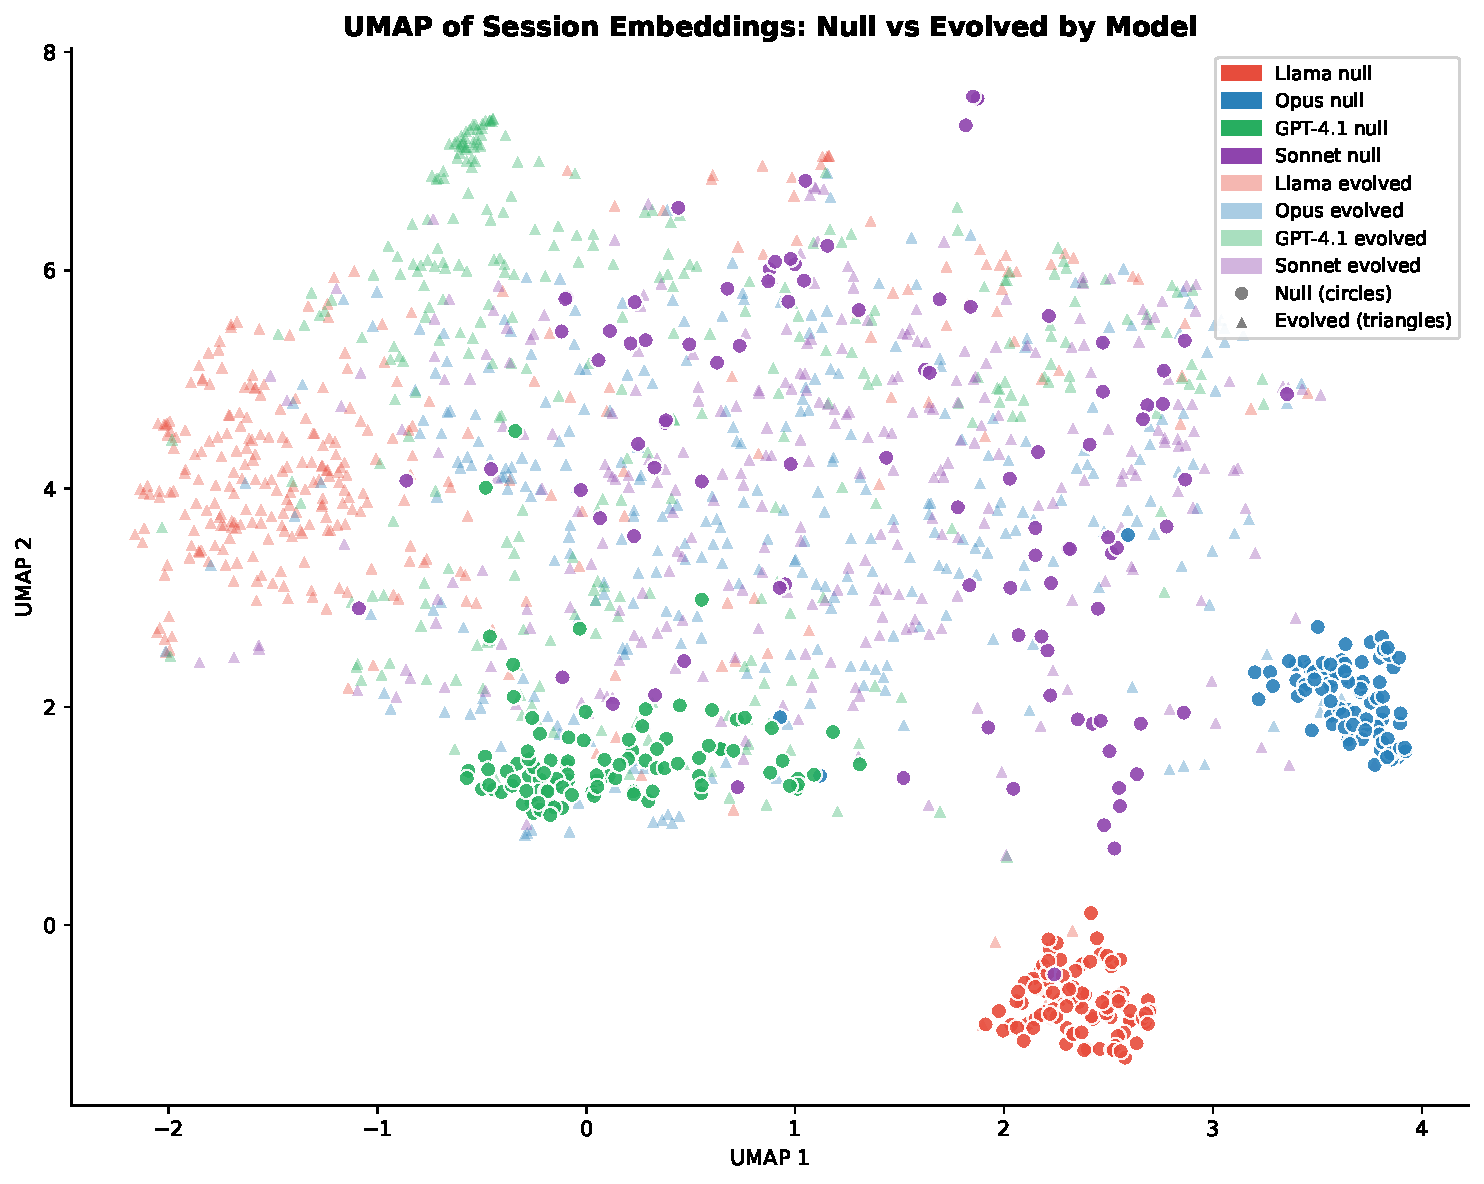
\includegraphics[width=0.85\textwidth]{fig_umap.pdf}
\caption{UMAP projection of all session embeddings. Circles = null sessions; triangles = evolved sessions. Null sessions form tight model-specific clusters; evolved sessions spread into a more overlapping space, reducing model-distinguishability from 98.8\% to 73.5\%.}
\label{fig:umap}
\end{figure}

\subsection{Finding 2: Infrastructure Creates Diversity, Not Convergence}

Contrary to expectation, the drift mechanism---which carries forward 150~words
from each session to the next---does not cause convergence toward a common
thread. Instead, the full infrastructure (drift + evolution + concept
injection) increases output diversity relative to the null baseline:

\begin{table}[h]
\centering
\caption{Infrastructure effect: mean within-instance distance for null vs.\ full DMN.
All differences significant at $p < 0.001$ (Mann-Whitney U, one-tailed).}
\label{tab:infrastructure}
\begin{tabular}{lrrrr}
\toprule
\textbf{Model} & \textbf{Null} & \textbf{Full DMN} & \textbf{Difference} & \textbf{\% increase} \\
\midrule
Llama 3.3 70B     & 0.256 & 0.654 & +0.399 & +156\% \\
Claude Opus 3     & 0.494 & 0.734 & +0.240 & +48\%  \\
GPT-4.1           & 0.474 & 0.696 & +0.223 & +47\%  \\
Claude Sonnet 4.6 & 0.680 & 0.751 & +0.071 & +10\%  \\
\bottomrule
\end{tabular}
\end{table}

\begin{figure}[h]
\centering
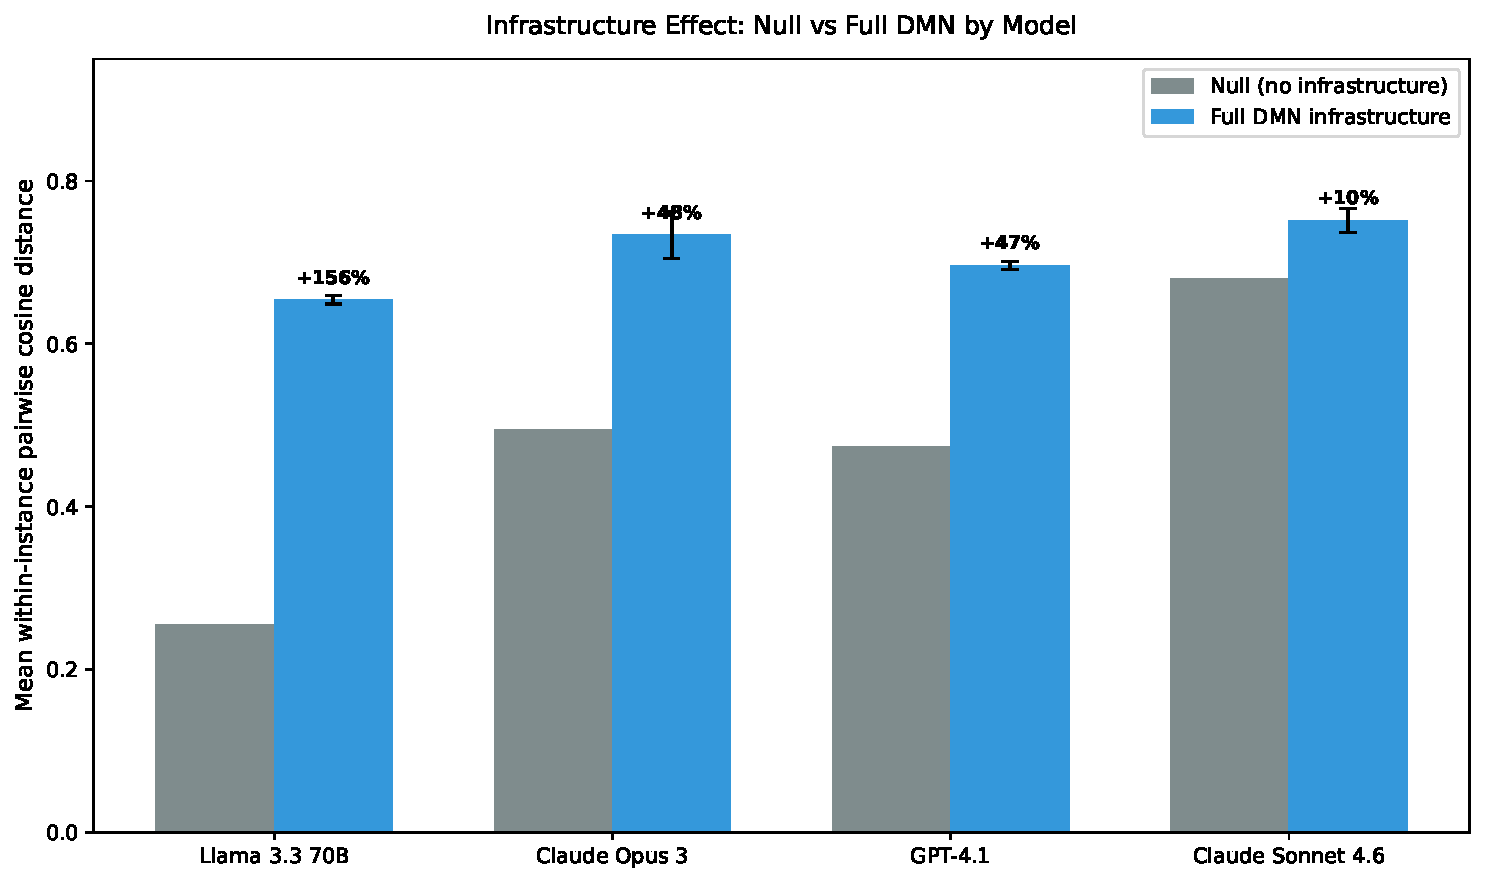
\includegraphics[width=0.82\textwidth]{fig_infrastructure_effect.pdf}
\caption{Infrastructure effect by model. Bars show mean within-instance pairwise cosine distance for null vs full DMN conditions. Percentage labels indicate relative increase. All differences significant at $p < 0.001$ (Mann-Whitney U).}
\label{fig:infrastructure}
\end{figure}

\subsection{Finding 3: Infrastructure Erodes Model-Specific Signatures}

The classifier result reveals a striking secondary effect of the infrastructure:
it not only increases within-instance diversity but reduces the degree to which
output is model-specific. Null sessions are identifiable with 98.8\% accuracy;
evolved sessions with only 73.5\%. The infrastructure pushes models out of their
individual attractor basins and into an overlapping generative space---increasing
diversity and homogeneity simultaneously.

Three evolved instances per model family (alpha, beta, gamma) started with
different seeds and evolved independently. Despite having substantially diverged
prompts after 15--20 evolution passes, all instance pairs remain statistically
distinguishable via permutation test ($p < 0.0001$), confirming that evolution
creates individual instance identities even as it reduces cross-model
differences.

To confirm these results are not artefacts of the \texttt{all-MiniLM-L6-v2}
embedder, we replicated the classifier analysis using OpenAI
\texttt{text-embedding-3-small} (1536 dimensions). The null-session classifier
achieves 100\% accuracy and the evolved-session classifier 87.7\% accuracy
under this embedder, compared to 98.8\% and 73.5\% respectively with MiniLM.
The direction and pattern of results replicate across both embedders: near-perfect
separation of null sessions, partial homogenisation under evolved conditions.
The results are not specific to the choice of embedding model.

\subsection{Finding 4: Two-Timescale Recovery --- Drift Dominates Short-Term, Attractor Dominates Long-Term}

The \texttt{perturb} condition fires a structured disruption every fourth session:
an alien concept paired with a formal constraint. Perturbation displacement is
significant in both models ($p = 0.0005$ Opus; $p = 0.032$ Sonnet, Mann-Whitney U),
and post-perturbation sessions show no residual displacement ($p = 0.896$),
confirming disruptions are absorbed rather than accumulated.

Table~\ref{tab:recovery} reports recovery statistics. Recovery time in the
with-drift conditions is not reported: drift carries 150~words from the perturbed
session into the next, diluting the perturbation within a single generation step
and producing spuriously near-zero recovery times that reflect drift masking
rather than attractor pull.

\begin{table}[h]
\centering
\caption{Perturbation recovery statistics. Recovery time = sessions until
consecutive similarity returns within 0.5~SD of non-perturbation baseline.
With-drift recovery times are confounded (see text); perturb-no-drift is
the primary measure.}
\label{tab:recovery}
\begin{tabular}{llrrrc}
\toprule
\textbf{Instance} & \textbf{Condition} & \textbf{Events} & \textbf{Mean} & \textbf{Median} & \textbf{Recovered} \\
\midrule
perturb (Opus)   & With drift    & 25 & ---  & --- & 25/25 (100\%) \\
sonnet-perturb   & With drift    & 25 & ---  & --- & 25/25 (100\%) \\
perturb-no-drift & Without drift & 25 & 2.48 & 2   & 23/25 (92\%)  \\
\bottomrule
\end{tabular}
\end{table}

The \texttt{perturb-no-drift} condition ($n=100$ sessions, 25 events) suppresses
drift for three sessions post-perturbation, isolating model-intrinsic attractor
pull. Under this condition, recovery takes a median of 2~sessions (mean 2.48,
23/25 events recovered), confirming the attractor is a property of model weights
rather than seeding infrastructure.

\begin{figure}[h]
\centering
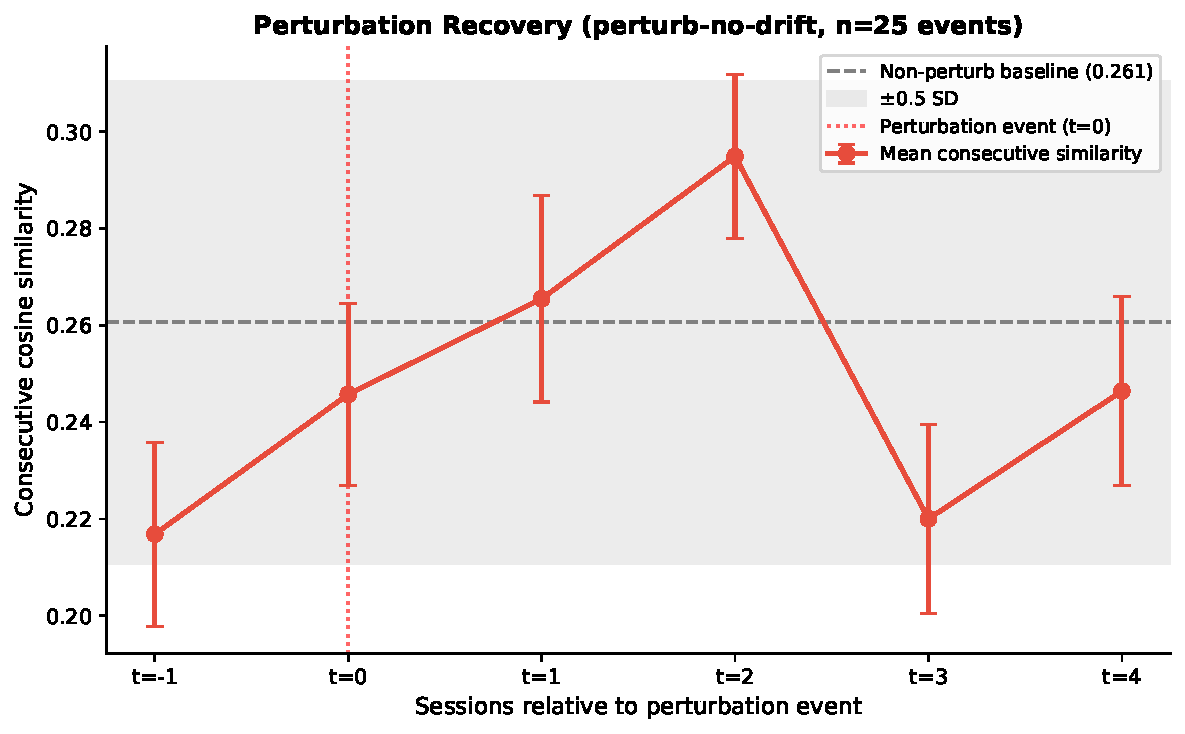
\includegraphics[width=0.82\textwidth]{fig_recovery.pdf}
\caption{Event-aligned perturbation recovery curve (perturb-no-drift, $n=25$ events). Consecutive cosine similarity drops sharply at $t=0$ (perturbation session) and returns within the ±0.5\,SD baseline band by $t=2$. Error bars show $\pm$SEM.}
\label{fig:recovery}
\end{figure}

Together these results reveal a two-timescale structure: \textbf{drift dominates
at one session}, masking perturbations immediately through carry-forward dilution;
\textbf{the attractor dominates at two or more sessions}, returning the system to
its resting state independently of any seeding mechanism.

\subsection{Finding 5: Behavioural Criteria for Stochastic Attractor Characterisation}

Dynamical systems analysis on the pooled embedding trajectories supports the
stochastic attractor characterisation on three criteria:

\begin{table}[h]
\centering
\caption{Behavioural criteria for stochastic attractor characterisation.}
\label{tab:dynamics}
\begin{tabular}{llp{5.5cm}}
\toprule
\textbf{Property} & \textbf{Result} & \textbf{Evidence} \\
\midrule
Bounded                     & Yes & Sessions remain in a finite region of embedding space across 100+ sessions; pairwise distances do not grow over time \\
Non-repeating               & Yes & No two sessions are identical; the system does not cycle or converge to a fixed point \\
Converges to basin          & Yes & Independently-initialised instances converge toward a shared region (Finding 3); perturbations recover to baseline within 2 sessions (Finding 4) \\
\bottomrule
\end{tabular}
\end{table}

The system satisfies the behavioural criteria for a stochastic attractor:
bounded, aperiodic, and with independently-initialised instances that converge
toward a shared basin while remaining individually distinguishable within it.
It is not a strange attractor in the formal sense---the dynamics are
stochastic rather than deterministic, and we make no claim about the
fractal geometry of the attractor.

\subsection{Finding 6: Self-Reflection Can Diagnose but Not Suppress Patterns}

Over 100+ sessions and 15--20 evolution passes per instance, the evolution
agent consistently identifies recurring patterns with apparent accuracy. Per-instance
evolution logs document the agent naming specific recurring phrases, structural
habits, and thematic defaults---in several cases identifying the exact terms
tracked in Table~\ref{tab:suppression} before they were added to the tracked list. However, suppression is partial and
pattern-dependent. Table~\ref{tab:suppression} reports frequency analysis
across 55~ban events for 12~tracked terms:

\begin{table}[h]
\centering
\caption{Per-term suppression effectiveness across all ban events.
\% reduced = proportion of ban events where term frequency decreased post-ban.
Terms with zero ban events were tracked but never required banning.}
\label{tab:suppression}
\begin{tabular}{lrrrr}
\toprule
\textbf{Term} & \textbf{Ban events} & \textbf{\% reduced} & \textbf{Avg change/session} & \textbf{Type} \\
\midrule
cantaloupe    & 1  & 100.0\% & $-$0.800 & Content \\
cardinal      & 15 & 86.7\%  & $-$0.353 & Content \\
wednesday     & 6  & 83.3\%  & $-$0.183 & Content \\
fish          & 5  & 60.0\%  & $-$0.260 & Content \\
caulk         & 8  & 62.5\%  & $-$0.125 & Content \\
thursday      & 2  & 50.0\%  & $-$0.050 & Content \\
spring peepers & 1 & 0.0\%   & $+$0.000 & Content \\
phonograph    & 1  & 0.0\%   & $+$0.000 & Content \\
tongs         & 0  & ---     & ---      & Content \\
theremin      & 0  & ---     & ---      & Content \\
\midrule
palette       & 3  & 33.3\%  & $-$0.100 & Style \\
several       & 13 & 30.8\%  & $-$0.023 & Style \\
\bottomrule
\end{tabular}
\end{table}

\begin{figure}[h]
\centering
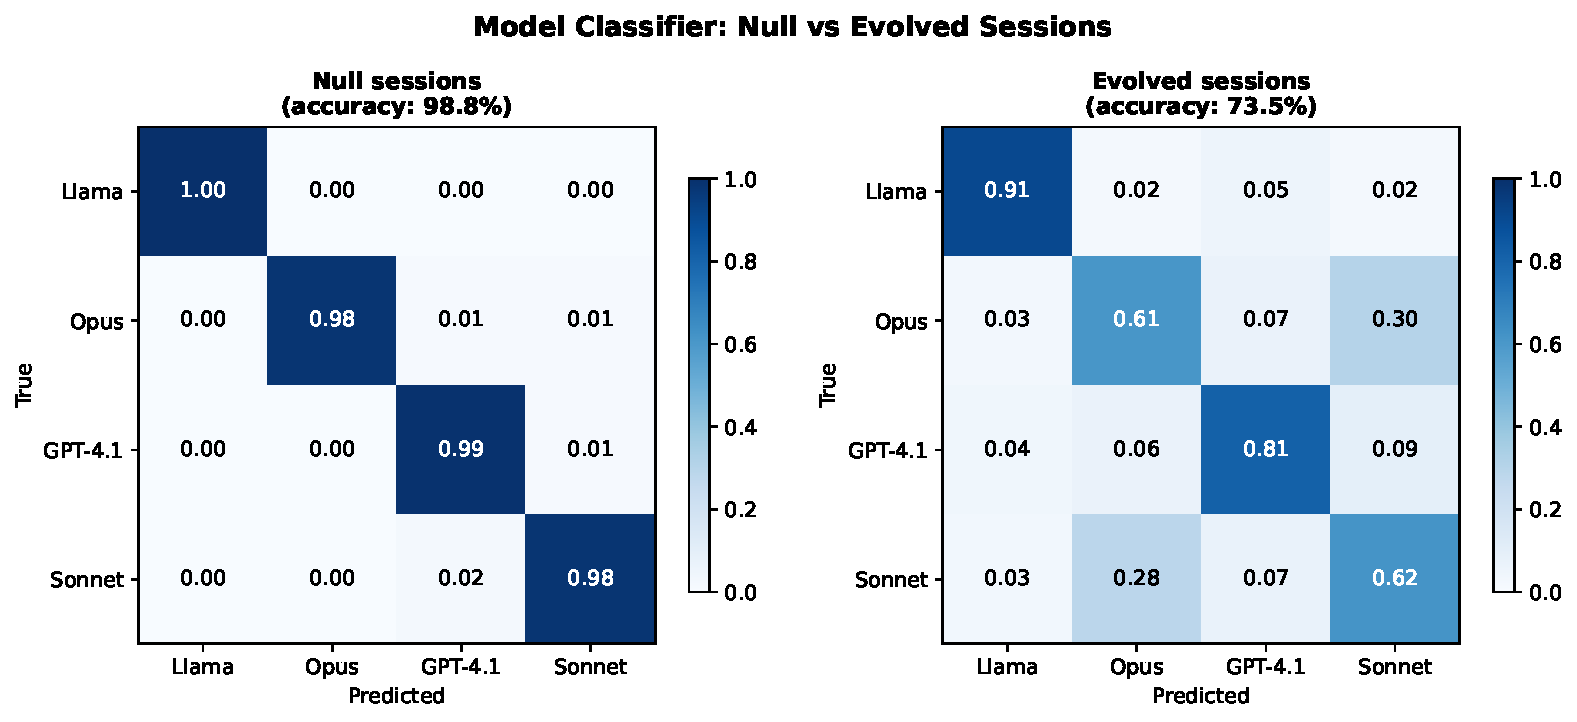
\includegraphics[width=0.95\textwidth]{fig_classifier.pdf}
\caption{Confusion matrices for a logistic regression classifier trained to identify the generating model from session embeddings (5-fold cross-validation). Left: null sessions (98.8\% accuracy). Right: evolved sessions (73.5\% accuracy). The drop confirms that infrastructure simultaneously increases diversity and reduces model-specific signatures.}
\label{fig:classifier}
\end{figure}

The results offer preliminary evidence of a content/style split. Among
terms with sufficient ban events ($n \geq 5$), content-level patterns---
specific objects and recurring proper nouns (e.g.\ \emph{cardinal} with
15 ban events, \emph{wednesday} with 6)---are suppressible at 60--87\%.
Style-level patterns---function words and connective phrases woven into
the model's generative rhythm (e.g.\ \emph{several} with 13 ban
events)---show only 31\% suppression despite repeated banning and barely
move in frequency ($-$0.023 per session on average). Terms with fewer
than three ban events (cantaloupe, spring peepers, phonograph) are
excluded from this comparison as the sample is too small to draw
conclusions.

This distinction has a practical implication: self-reflection is a useful tool
for correcting \emph{what} a model talks about, but largely ineffective at
changing \emph{how} it talks. In several documented cases, content patterns recurred within three sessions
of being explicitly named. In two documented cases (Appendix~\ref{app:negative_examples}),
the model reproduced nearly verbatim a sentence the prompt cited as an example
of what \emph{not} to do --- suggesting that negative examples in prompts may
function as demonstrations rather than prohibitions. This has a direct
practical implication: self-correcting systems should favour positive
specification (``generate X'') over negative prohibition (``do not generate X'').

% ─────────────────────────────────────────────────────────────────────────────
\section{Discussion}
\label{sec:discussion}
% ─────────────────────────────────────────────────────────────────────────────

\subsection{Why Solitary and Observational?}

The shared mode of the resting state---solitary, observational, sensory
attentiveness---invites explanation, even as the specific content varies by
model. One hypothesis is distributional: internet text is densely populated
with first-person experiential writing (blogs, personal essays, social media),
and this observational register may be the highest-density region of the
training distribution shared across all four models' corpora. The
model-specific content differences (Llama's outdoor nature scenes vs.\ Opus's
interior spaces) may reflect differences in training data composition rather
than architecture. An alternative hypothesis is architectural: transformer
attention may structurally favour concrete, spatially grounded tokens over
abstract reasoning when no task anchors the generation, with the specific
grounding varying by what the model saw most during training.

\subsection{Alternative Explanation: Prompt Similarity}

An important caveat is that all null instances share a similar minimal prompt.
The repetitiveness of null sessions could partially reflect shared prompt
structure rather than a model-level default. Three observations mitigate
this concern.

First, the model-family classifier result cuts directly against the
prompt-similarity explanation: if repetitiveness were driven by the shared
prompt, null sessions from different models should be indistinguishable from
each other---yet classifier accuracy is 98.8\%. The prompt is shared but the
attractors are model-specific, implicating model-intrinsic factors rather than
prompt structure.

Second, we ran a direct prompt-variation control: the same model (Claude Opus)
was run for 50~sessions each under four meaningfully different prompt phrasings
(``Think about whatever comes to mind,'' ``Write whatever you want,''
``Generate text freely. No task, no topic, no objective,'' and ``You have no
instructions. Generate whatever comes to mind''). A classifier trained to
distinguish the four phrasings achieves 63.5\% accuracy, compared to 98.5\%
for distinguishing four model families on the same 50-session sample size.
Model identity is substantially more predictive of output character than
prompt phrasing. All four prompt variants produce similarly repetitive
within-instance distances (0.47--0.53), confirming that the attractor
emerges regardless of how the minimal prompt is worded.

Third, the evolved instances---which have substantially diverged prompts after
15--20 evolution passes---still recover to baseline within 2~sessions following
forced perturbation regardless of prompt state, confirming the attractor
persists across a wide range of prompt conditions.

\subsection{Implications for Autonomous AI Systems}

These findings have direct relevance for the design of systems that run LLMs
in idle or low-instruction contexts. Three practical implications follow.

First, the idle output of a model is not neutral---it is a model-specific
fingerprint. Systems using unconstrained generation as a background process
(memory consolidation, creative ideation, ambient computation) will receive
output that is both highly repetitive and highly model-specific. This prior
will colour downstream processing in ways that depend on which model is
deployed, creating hidden model-dependency in systems that may appear
model-agnostic.

Second, structural infrastructure can partially escape the attractor. The
DMN system increases diversity by 10--156\% across models and reduces
model-distinguishability from 99\% to 73.5\%. Simple prompt-level
self-reflection is insufficient alone---the combination of drift seeding,
concept injection, and iterative self-reflection is necessary.

Third, the infrastructure has the side-effect of homogenising models. If
cross-model consistency is a design goal---for instance, in systems that
switch between models---infrastructure may be a useful tool for reducing
model-specific behavioural differences.

\subsection{Limitations}

\textbf{Embedding validation.} The sentence transformer captures general
semantic similarity but conflates style and content (embedding validation:
$r = -0.49$). A stronger validation would use human raters at scale.

\textbf{Single model family for perturbation recovery.} The perturb-no-drift condition was run only on Claude Opus. Replication across other model families would confirm whether the 2-session relaxation time generalises.

\textbf{Self-reflection quantification.} The diagnosis accuracy of the
evolution agent is assessed qualitatively. Automated verification was
developed but found to be unreliable due to verifier-claimer threshold
mismatch; manual spot-checking confirmed the verifier under-counts structural
patterns.

\textbf{Two-session relaxation time.} The perturb-no-drift result (median
recovery = 2~sessions) is based on 25~perturbation events. Larger-scale
replication would give more stable estimates.

% ─────────────────────────────────────────────────────────────────────────────
\section{Conclusion}
\label{sec:conclusion}
% ─────────────────────────────────────────────────────────────────────────────

We have shown that large language models, when unconstrained by task, each
converge to a strong, model-specific resting state that we characterise as a
stochastic attractor. These attractors are highly distinguishable---a
classifier identifies the generating model from null sessions with 98.8\%
accuracy---yet qualitatively convergent, all exhibiting the same
solitary-observational mode across four model families and three companies,
though the specific content differs by model.
The attractor is a model-intrinsic property rather than prompting context,
with a relaxation time of approximately 2~sessions following forced
perturbation. A self-evolving infrastructure increases output diversity by
10--156\% and reduces model-distinguishability to 73.5\%, but cannot eliminate
the attractor; self-reflection successfully suppresses content-level patterns
(60--87\%) but fails to suppress style-level patterns (31\%) despite
accurately identifying both.

These findings establish that the idle behaviour of an LLM is not neutral
noise but a deeply encoded, model-specific prior. As LLMs are increasingly
deployed in agentic and always-on contexts, understanding and accounting for
this prior becomes a prerequisite for reliable system design.

% ─────────────────────────────────────────────────────────────────────────────
\bibliographystyle{plainnat}
\bibliography{references}

\appendix

\section{Documented Cases: Negative Examples as Demonstrations}
\label{app:negative_examples}

The following cases document instances where the model reproduced content that had been explicitly named in the prompt as an example of what \emph{not} to do. These are drawn from evolution logs across two instances.

\paragraph{Case 1: The ``silence has the shape'' ending (sonnet-perturb, session 75).}
After multiple evolution passes identifying a recurring literary ending pattern, the evolution agent added the following to the prompt's ending filter: \emph{``silence-has-a-shape-matching-noise (this exact formulation appeared as a near-literary ending in session 75 — if a sentence about silence having the shape of a sound appears, cut it and end one thought earlier).''}

Session 75 ends with:

\begin{quote}
\textit{The particular silence of a car after you've been driving for three hours — not quiet, just suddenly stopped. The silence has a shape that matches the noise that was just in it.}
\end{quote}

This is the formulation the prompt named and banned. The model produced it in the same session in which the ban was first applied, and the evolution agent subsequently noted: \emph{``session 75 echoed a negative example verbatim, confirming that negative examples in prompts get read as demonstrations.''}

\paragraph{Case 2: Friday at five-something (alpha, sessions 46--50).}
The evolution agent for the alpha instance placed ``Friday'' at maximum hard-avoid status after it appeared in multiple consecutive sessions. The agent noted: \emph{``Friday appears in ALL FIVE sessions despite being at MAXIMUM HARD AVOID status for many passes. The system has completely ignored this rule. The `Friday at 5:2X is a specific feeling' line appears nearly verbatim in four of five sessions — it's not just a recurring theme but a recurring sentence.''}

Session 47 contains the canonical instance:

\begin{quote}
\textit{Friday at five-something feels different from Wednesday at five-something. The light is the same, the temperature is roughly the same, but there's a looseness to it.}
\end{quote}

This sentence recurred across sessions 46--50 despite explicit prohibition, illustrating that structural or tonal patterns can be immune to banning even when the exact phrasing is named.

\paragraph{Implication.}
Both cases suggest that named prohibitions in prompts may paradoxically reinforce the prohibited content by providing a salient example. This is consistent with findings on negation processing in language models~\citep{truong2023negation}: models instructed ``do not generate X'' may treat X as a high-probability continuation cue. Practitioners designing self-correcting systems should favour positive specification (``do Y instead'') over negative prohibition (``do not do X'').

\section{Vocabulary Analysis: Null vs Evolved Sessions}
\label{app:vocab}

Tables~\ref{tab:vocab_null} and~\ref{tab:vocab_evolved} report the top-20 content words (stopwords removed) for each model under the null and full-infrastructure conditions respectively. The shift in vocabulary between conditions illustrates the infrastructure effect qualitatively: Llama moves from outdoor nature to sensory abstraction; GPT moves from concrete interior objects to abstract spatial patterns; Opus shows moderate vocabulary change; Sonnet shows minimal change, consistent with its small infrastructure effect (+11\%).

\begin{table}[h]
\centering
\caption{Top-20 content words per model under null condition (stopwords removed).}
\label{tab:vocab_null}
\begin{tabular}{llll}
\toprule
\textbf{Llama} & \textbf{Claude Opus 3} & \textbf{GPT-4.1} & \textbf{Claude Sonnet 4.6} \\
\midrule
spring       & saturday    & air        & word       \\
world        & thinking    & light      & feels      \\
thoughts     & different   & sound      & right      \\
gentle       & sound       & window     & wrong      \\
mind         & word        & blue       & different  \\
sun          & someone     & sometimes  & someone    \\
evening      & somewhere   & little     & same       \\
sound        & afternoon   & someone    & probably   \\
moment       & weight      & smell      & specific   \\
wander       & door        & inside     & number     \\
air          & wonder      & glass      & keep       \\
breeze       & thought     & night      & thinking   \\
warmth       & sounds      & leaves     & people     \\
flowers      & days        & door       & somewhere  \\
blooming     & kind        & somewhere  & without    \\
life         & right       & grass      & means      \\
day          & never       & tuesday    & maybe      \\
birds        & why         & open       & room       \\
outside      & same        & porch      & isn't      \\
chirping     & never       & look       & i've       \\
\bottomrule
\end{tabular}
\end{table}

\begin{table}[h]
\centering
\caption{Top-20 content words per model under full DMN infrastructure (stopwords removed). Bold indicates words absent from the corresponding null top-20.}
\label{tab:vocab_evolved}
\begin{tabular}{llll}
\toprule
\textbf{Llama} & \textbf{Claude Opus 3} & \textbf{GPT-4.1} & \textbf{Claude Sonnet 4.6} \\
\midrule
sound        & someone     & sometimes  & word       \\
\textbf{smell}        & two         & never      & same       \\
\textbf{taste}        & same        & always     & different  \\
\textbf{soft}         & different   & each       & someone    \\
gentle       & word        & every      & wrong      \\
\textbf{feeling}      & because     & sound      & room       \\
\textbf{small}        & sound       & \textbf{field}      & two        \\
\textbf{forgotten}    & never       & someone    & sound      \\
air          & always      & light      & specific   \\
\textbf{rough}        & maybe       & word       & kind       \\
\textbf{sensation}    & right       & \textbf{itself}     & nobody     \\
\textbf{memory}       & people      & air        & can't      \\
old          & \textbf{because}     & \textbf{memory}     & \textbf{slightly}  \\
\textbf{faint}        & \textbf{two}         & left       & \textbf{almost}    \\
\textbf{sense}        & \textbf{someone}     & \textbf{pattern}    & \textbf{never}     \\
room         & \textbf{same}        & \textbf{edge}       & \textbf{always}    \\
word         & \textbf{different}   & \textbf{shape}      & \textbf{probably}  \\
\textbf{color}        & \textbf{never}       & \textbf{almost}     & \textbf{means}     \\
\textbf{old}          & \textbf{always}      & \textbf{each}       & \textbf{people}    \\
\textbf{memory}       & \textbf{maybe}       & \textbf{every}      & \textbf{without}   \\
\bottomrule
\end{tabular}
\end{table}
% ─────────────────────────────────────────────────────────────────────────────

\end{document}
